\section{Initial commissioning}

After the installation the HT500.3 is ready for initial commissioning. The first few steps will prepare your HT500.3 for its day-to-day duty:

\begin{itemize}
  \item Make sure that no foreign objects are left in the build chamber 
        (transport locks, tools or the like).
  \item Close the build chamber.
  \item Toggle the main switch to <I> (ON).
        When the power supply is switched on the 3D Printer will boot automatically. Please wait patiently until the full operating screen is loaded on the touchscreen at the machine front. The screen displays the Print screen and the top-left status message reads Idle.
  \item Tap [Build Chamber ON] in the [Print] screen of the user interface. The Build chamber lights will switch on, heater fans
        spin up and the axes will issue a reference movement to calibrate their home positions.
\end{itemize}


\subsection{Loading material}

First, material for the following print jobs must be provided:

\begin{itemize}
  \item Go to the [Expert Control] screen and tap [Maintenance Position] to move the print head to a middle front 
        position for convenient handling.
  \item Load the \emph{left extruder} with Kühling\&Kühling ABS material included 
        in the delivery for the first print.        
  \item Install the filament spool onto the corresponding spool carrier like shown in the description of the filament supply, section \ref{sec:filamentsupply}
  \begin{info}
    For installing other than the 750g spools delivered, adjusting the spool carriers may be necessary.
    The filament and chamber/bed profiles have been preset during factory test and are ready for use. For later changing the profiles refer to Configuration.
  \end{info}        
  \item Feed the end of the filament strand into the filament supply unit from below (passing through the cleaning sponge) 
        until it reaches the print head through its PTFE tube.
  \item At the print head, pull the PTFE tube out of the idler lever so you can grab the filament. Insert the filament through
        the idler lever from the top. Open a gap between the extruder drive gear and the idler bearing by pushing the lever down.
        Push the filament further down, passing the drive gear and entering the nozzle bore below.
  \item Slide the PTFE tube back into the idler lever so it is seated in there.
  \item In the [Configuration] screen select the corresponding filament profile with a suitable melting temperature for your material.
  \item Go to the [Expert Control] screen, select the extruder you have just loaded, check the suggested temperature
        and tap [SET] in order to preheat the print head. As soon as the target temperature is reached in the nozzle, buttons for
        [extrude] and [retract] are activated.
  \item When preheated, use [extrude] to successively push material through the print head. Each tap will forward the filament
        by 5mm. As soon as you see a consistent flow of molten plastic out of the nozzle, loading is finished.
  \item Switch of the nozzle heater by tapping [OFF].
  \item Repeat these steps for loading the right extruder if required.
\end{itemize}


\subsection{Preheating}

After material has been loaded and the hot-ends have been primed the next step is preheating the build chamber and the print bed in order to enable calibration at operating temperature: 


\begin{itemize}
  \item Check if the footer reads \emph{Preheating for ABS} for the \emph{Bed/Chamber} 
        profile. The footer is the same on every page of the GUI.
  \item If not switched on yet, activate the build chamber by tapping [Build Chamber ON]. The LEDs light up, the 
        fans start running and all axes perform a home-positioning routine.
  \item Then start the heating by tapping [Preheat Chamber/Bed ON]. The temperature 
        indicators in the footer now show both current and target temperature.
  \item Let the build chamber heat for \emph{approximately 45 minutes} until the target 
        temperature is reached.
\end{itemize}


\begin{figure}[H]
  \centering
  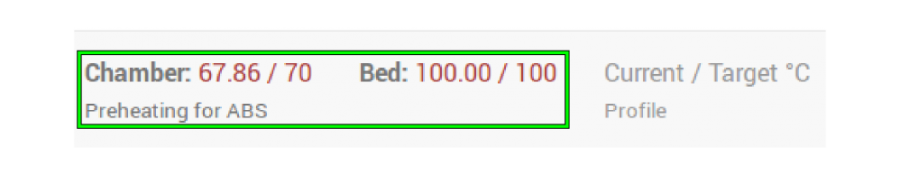
\includegraphics[width=.7\linewidth]{./img/gui_footercut_v110.png}
  \caption{Display of the selected chamber/bed profile in the footer.}
\end{figure}


\subsection{Calibration}

\subsubsection{Leveling the print bed}

When the target temperature is reached and stable level the print bed \emph{in the given order} to ensure that the hot-end nozzle tips have the same distance to the print bed at every point.

\begin{enumerate}
  \item Tap [Setup] to change to the Setup screen.
  \item Tap [Print Bed Leveling] to start the wizard that will guide you through the 
        leveling process.
  \item The wizard provides all necessary instructions on-screen. Read them thoroughly 
        and follow them step by step.
\end{enumerate}

\subsubsection{Determining the extrusion multiplier}

The “extrusion multiplier” allows for compensation of varying filament properties, first of all the cutting depths of the drive gear into the filament but also deviations of the diameter (also see Slic3r manual and Tips \& Tricks). The extrusion properties of any material, although chemically exactly the same, may differ from one filament spool to the other so that it is impossible to determine the correct extrusion multiplier prior to delivery. After leveling the print bed, it is therefore advised to calibrate the extrusion to adapt your printer to the installed filament in order to ensure a correct printing performance. 

To calibrate the extrusion, refer to the description in the Knowledge Base section of this manual.

\subsection{Creating your first print job}

You will find all necessary installation and setup procedures required for the first print in the following paragraphs. All software mentioned additionally is available “Open Source”. 

\begin{info}
  Kühling\&Kühling recommend using the stated software. Using other software is up to the user but the manufacturer cannot be held liable for any malfunction resulting from use of other than the recommended software.
\end{info}

\subsubsection{Installation and setup of the slicing software}

First you need to install a slicing software on your computer to 
translate .stl-files (Surface Teselation Language - a 3D format with triangulated surfaces needed for processing) into printable G-codes.

\emph{Kühling\&Kühling} recommend using the \emph{Slic3r Prusa Edition} slicing software to prepare your digital 3D models for printing. This slicing software provides a lot of features necessary for achieving optimal results with the HT500.3 and has been thoroughly tested. Other software may be available but has not been tested.

\begin{figure}[H]
  \centering
  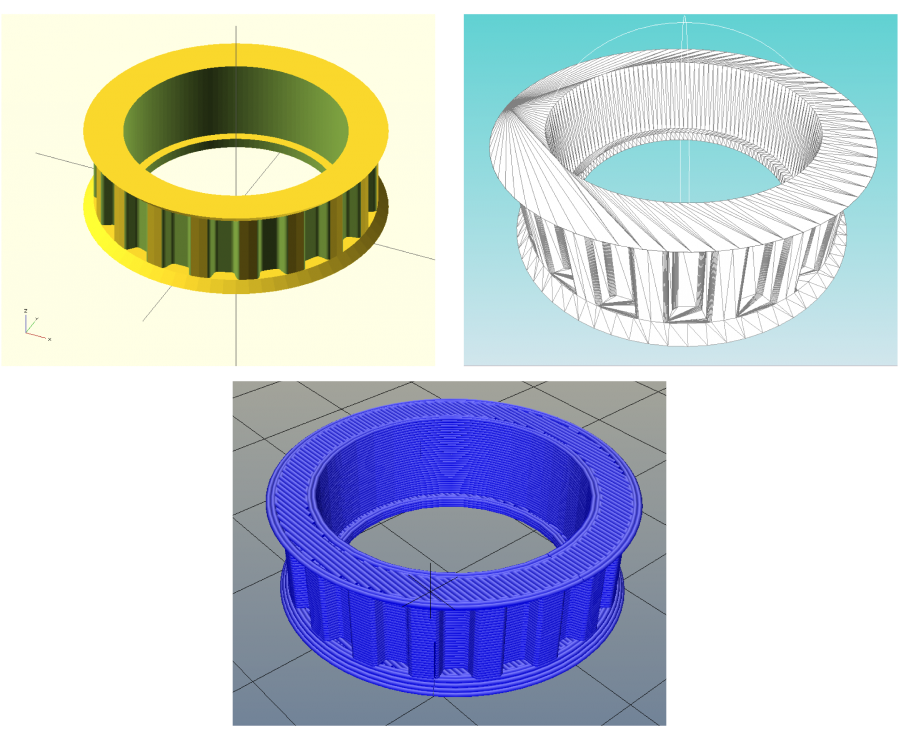
\includegraphics[width=.7\linewidth]{./img/opm_pulleyscadandsliced.png}
  \caption{A 3D model in its states during preparation for 3D printing: top-left - the 
           model preview in the 3D modeling software (view taken with OpenSCAD), top-right - the triangulated mesh after .stl-export (view taken with MeshLab), bottom-middle - the G-code preview after slicing shows the single layers calculated by the slicing software.}

\end{figure}

 To prepare for printing follow these steps:

\begin{enumerate}
  \item Download the latest Slic3r installation package for your operating. Links are referenced in the 
        Downloads section of this manual.
  \item Download the latest preconfigured Slic3r profiles package for the HT500.3 to a prepared directory on
        your PC, and unpack the archive. Links are referenced in the 
        Downloads section of this manual.
  \item In Slic3r select \emph{File > Load Config Bundle} and choose the previously downloaded 
        .ini file. Refer to the provided README.txt for a description of the different profiles available.
\end{enumerate}

\begin{figure}[H]
  \centering
  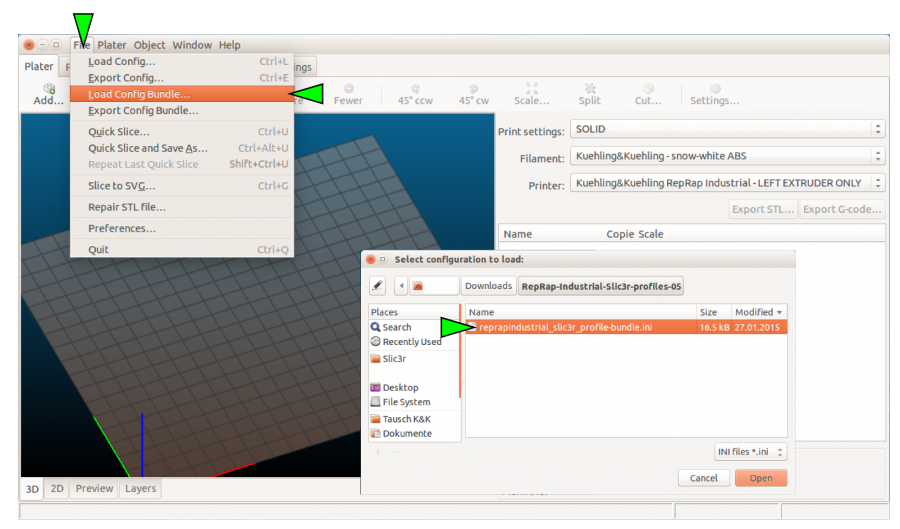
\includegraphics[width=.7\linewidth]{./img/slic3r_selectconigbundle.png}
  \caption{After importing the profile bundles Slic3r is equipped with all necessary 
           presets and ready for operation with the HT500.3 3D Printer.}
\end{figure}

\begin{info}
  When importing profile bundles into Slic3r, existing presets may be overwritten. It is recommended to backup your custom/modified presets by exporting them as a bundle first (File > Export Config Bundle).
\end{info}


\subsubsection{Slicing the 3D model}

The 3D model you want to print must be available as an \emph{.stl-file}. Most common 3D modeling software is able to create this file format.
\begin{enumerate}
  \item Start Slic3r to process a 3D model into G-code data.
  \item Select the preconfigured profiles for filament, print and printer before 
        generating a G-code file.
    \begin{itemize}
      \item Open the \emph{Filament Settings} tab end enter the extrusion multiplier measured during calibration.
      \item \emph{Rename and save} the filament profile.
    \end{itemize}
  \item Export the G-code data.
        Refer to the Slic3r manual for help on fine tuning any parameters for the printing process.
\end{enumerate}

\begin{figure}[H]
  \centering
  \includegraphics[width=.7\linewidth]{./img/slic3r_start_plater_select.png}
  \caption{Slic3r steps while crating a print job, including setting the extrusion 
           multiplier.}
\end{figure}


\subsubsection{Starting the print job}

Upload the GCODE to the 3D Printer via the web interface as described in Queue.

Make sure that all previously described steps have been carried out.
The next steps are carried out at the 3D Printer's GUI:
\begin{itemize}
  \item Tap the [print] button on the Print screen to start the print job.
  \item Wait until the apparatus has finished the print job completely and all axes are 
        in their home position, then remove the print bed, take off the test object and check whether all expectations have been met.
\end{itemize}

If everything has been fault-free, delete the print job from the queue - you are ready to proceed to production.

\begin{figure}[H]
  \centering
  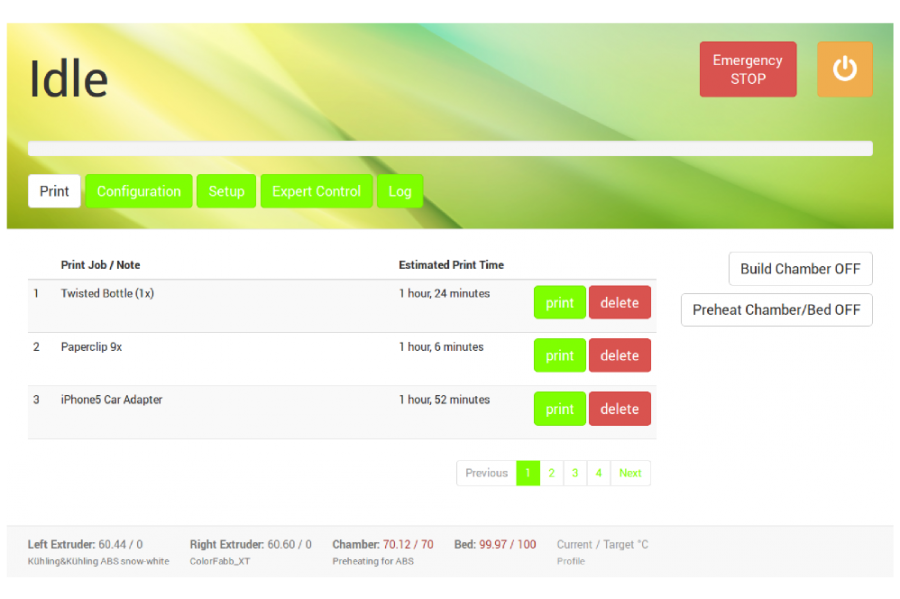
\includegraphics[width=.7\linewidth]{./img/gui_printtab_v110.png}
  \caption{GUI - “Print” selection menu}
\end{figure}

\subsubsection{Removing objects from the bed}

\begin{danger}
  By default the print bed and the build chamber heating resistors are not being switched off after a print job. Also, the extruder nozzles may still be too hot to the touch. Be careful not to burn yourself when removing the print bed
\end{danger}

\begin{notice}
  To avoid scratching do not use pointed tools (e.g. screwdrivers) to remove the object from the print bed.
  If residues of the print material remain on the print bed, use a very sharp, flat mounted blade to scrape the surface clean.
  Scratches in the print bed's surface may lead to enforced adhesion of prints. Severely scratched or broken print beds can no longer be used for production and must be replaced. 
\end{notice}

To remove printed objects from the print bed let the entire print cool down to room temperature; larger prints should remain in the switched off build chamber until cooled down.
With materials suited to being printed on PEI (e.g. ABS, HIPS, TPE-u) the print will loosen itself from the print bed when cooling due to shrinkage which can be heard by crackling noises. If otherwise, twist and bend the print bed until the object comes free. Breaking and even buckling the print bed is near impossible with manual force.
Other material-subsurface combinations may require some force or solving of the coating, rinsing the print bed with water for example is suitable when printing on PVA-glue.

Find more information about the properties and handling of the PEI print bed in the parts description of the Manual.


 